\section{Motivation}

% add outline page with current section highlighted.
\begin{frame}{Outline}{ $ \null $ }
	\tableofcontents[currentsection]
	%\tableofcontents[currentsection,currentsubsection]
\end{frame}

\subsection{Differences between Human and Robot}

\begin{frame}{Humans and Robots Think Differently}{Motivation}

\begin{columns}
\column{0.4\textwidth}
\begin{block}{ Human's Brain }
\centering
{\bf Krang}
\begin{figure}
	\centering
	\includegraphics[width=.7\linewidth]{figure/human_brain}
\end{figure}
\end{block}	
\column{0.4\textwidth}
\begin{block}{ Robot's Chip }
\centering
{\bf Baymax}
\begin{figure}
	\centering
	\includegraphics[width=.7\linewidth]{figure/baymax_and_chip}
\end{figure}
\end{block}	
\end{columns}

\end{frame}

\begin{frame}{Qualitative vs Quantitative}{Motivation}

\begin{block}{}

Humans and robots process and express in different way.

\end{block}

\begin{columns}
\column{0.47\textwidth}

\begin{block}{ Qualitative }

\begin{minipage}[t][5cm][t]{.9\textwidth}

\centering
{\bf ``I am at the east of the TMCB.''}

\begin{figure}
	\centering
	\includegraphics[width=\linewidth]{figure/human_localization_rough}
\end{figure}
\end{minipage}

\end{block}

\column{0.47\textwidth}

\begin{block}{ Quantitative }

\begin{minipage}[t][5cm][t]{.9\textwidth}

\centering
{\bf Location $( 35.7 , 47.5 )$ \\ Orientation 72.1$^{\circ}$}

\begin{figure}
	\centering
	\includegraphics[width=\linewidth]{figure/robot_localization}
\end{figure}
\end{minipage}

\end{block}

\end{columns}

\end{frame}

\begin{frame}{Qualitative vs Quantitative}{Motivation}

\begin{columns}
\column{0.47\textwidth}

\begin{block}{ Qualitative }

\begin{minipage}[t][5cm][t]{.9\textwidth}

\centering
{\bf ``An apple is good, and a banana is better.''}

\begin{figure}
	\centering
	\includegraphics[width=.45\linewidth]{figure/human_preference}
\end{figure}
\end{minipage}

\end{block}

\column{0.47\textwidth}

\begin{block}{ Quantitative }

\begin{minipage}[t][5cm][t]{.9\textwidth}

\centering
{\bf {\sc \bf Utility}( banana ) $ = 100 $ \\ {\sc \bf Utility}( apple ) $ = 80 $ }

\begin{figure}
	\centering
	\includegraphics[width=.6\linewidth]{figure/robot_preference}
\end{figure}
\end{minipage}

\end{block}

\end{columns}

\end{frame}

\begin{frame}{Human-Robot Collaboration}{Motivation}

\begin{columns}
\column{0.4\textwidth}
\begin{block}{ Human's Role }
\begin{minipage}[t][1.2cm][t]{.9\textwidth}
\centering
\begin{itemize}
\item {\bf Coach}
\item {\bf Player}
\end{itemize}
\end{minipage}
\end{block}	
\column{0.4\textwidth}
\begin{block}{ Robot's Role }
\begin{minipage}[t][1.2cm][t]{.9\textwidth}
\centering
\begin{itemize}
\item {\bf Player}
\end{itemize}
\end{minipage}
\end{block}	
\end{columns}

\begin{figure}
	\centering
	\includegraphics[width=.7\linewidth]{figure/human_robot_collaboration}
\end{figure}

\end{frame}

\begin{frame}{Human-Robot Collaboration}{Motivation}

\begin{figure}
	\centering
	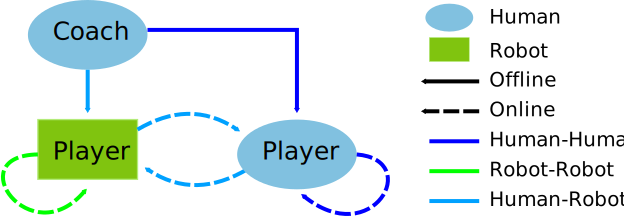
\includegraphics[width=.7\linewidth]{figure/team_info_flow}
\end{figure}

\end{frame}

\begin{frame}{From Quantitative to Qualitative}{Motivation}

\begin{columns}
\column{0.45\textwidth}
\begin{block}{ Location }
\begin{minipage}[t][4cm][t]{\textwidth}
\centering

\begin{itemize}
\item softmax regression
\end{itemize}
\begin{figure}
	\centering
	\includegraphics[width=.9\linewidth]{figure/softmax_func}
	\caption{ \tiny{ {\it Sample et al.} "An experimental evaluation of Bayesian soft human sensor fusion in robotic systems."  2012 AIAA Guidance, Navigation and Control Conference.} }
\end{figure}

\end{minipage}
\end{block}	
\column{0.45\textwidth}
\begin{block}{ Preference }
\begin{minipage}[t][4cm][t]{\textwidth}
\centering

\begin{itemize}
\item fuzzy membership function
\end{itemize}
\begin{figure}
	\centering
	\includegraphics[width=.9\linewidth]{figure/membership_func}
	\caption{ \tiny{ {\it Wang et al. } ``A comprehensive decision support model for the evaluation of eco-designs.'' Journal of the Operational Research Society 2013. } }
\end{figure}

\end{minipage}
\end{block}	
\end{columns}

\end{frame}

\begin{frame}{From Qualitative to Quantitative?}{Motivation}

\begin{columns}
\column{0.4\textwidth}
\begin{minipage}[t]{.9\textwidth}
\begin{block}{ Location }
\centering
\begin{figure}
	\centering
	\includegraphics[width=.4\linewidth]{figure/question_mark}
\end{figure}
\end{block}
\end{minipage}
\column{0.4\textwidth}
\begin{minipage}[t]{.9\textwidth}
\begin{block}{ Preference }
\centering
\begin{figure}
	\centering
	\includegraphics[width=.4\linewidth]{figure/question_mark}
\end{figure}
\end{block}
\end{minipage}	
\end{columns}

\begin{block}{\bf Approach}

\begin{center}
\begin{minipage}[t]{.8\textwidth}
\begin{block}{}
\begin{itemize}
\item Probabilistic model
\end{itemize}
\end{block}
\end{minipage}
\end{center}

\begin{center}
\begin{minipage}[t]{.8\textwidth}
\centering
\begin{block}{}
\begin{itemize}
\item Posterior method
\end{itemize}
\end{block}
\end{minipage}
\end{center}

\end{block}

\end{frame}


